\documentclass{beamer}
\usepackage[utf8]{inputenc}
\usepackage[T1]{fontenc}
\usepackage{lmodern}
\usepackage{graphicx}
\usepackage{amsmath,amsfonts,amssymb}
\usepackage{tikz}

\begin{document}
  \title{OPAM for Coq}
  \author{Guillaume Claret}
  \date{October 23, 2014 - Coq Working Group}
  \maketitle

  \section*{Need}
  \begin{frame}
    \frametitle{The need for a package manager}
    Even if there seem to be more and more developers:
    \begin{itemize}
      \item few user developments are reused
      \item \emph{contribs} mechanism, but outdated and centralized
      \item no simple / uniform way to install a foreign library
    \end{itemize}
    A lot of time is lost. What other programming languages have:
    \begin{center}
      \emph{A package manager.}
    \end{center}
  \end{frame}

  \section*{Plan}
  \begin{frame}
    \tableofcontents
  \end{frame}

  \section{OPAM}
  \begin{frame}
    \frametitle{OPAM}
    \begin{center}
      
\includegraphics[width=4cm]{images/opam}
    \end{center}
  \end{frame}
  \begin{frame}
    \frametitle{OPAM: the package manager of OCaml}
    We will use OPAM.

    Why?
    \begin{itemize}
      \item OCaml people are our closest cousins
      \item some Coq developments depend on OCaml packages
    \end{itemize}
    What it is?
    \begin{itemize}
      \item a tool made by OCaml Pro
      \item 772 OCaml packages today
      \item dependency management based on the Mancoosi project
    \end{itemize}
  \end{frame}
  \begin{frame}
    \frametitle{What we have}
    \begin{itemize}
      \item a website (not online yet)
      \item four repositories: \emph{stable}, \emph{testing}, \emph{unstable}, \emph{coqs}.

        Hosted on \url{https://github.com/coq}.
      \item a bench system

        Hosted on \url{https://github.com/coq-bench}.
    \end{itemize}
  \end{frame}

  \section{Demo}
  \begin{frame}
    \frametitle{Demo}
    \begin{center}
      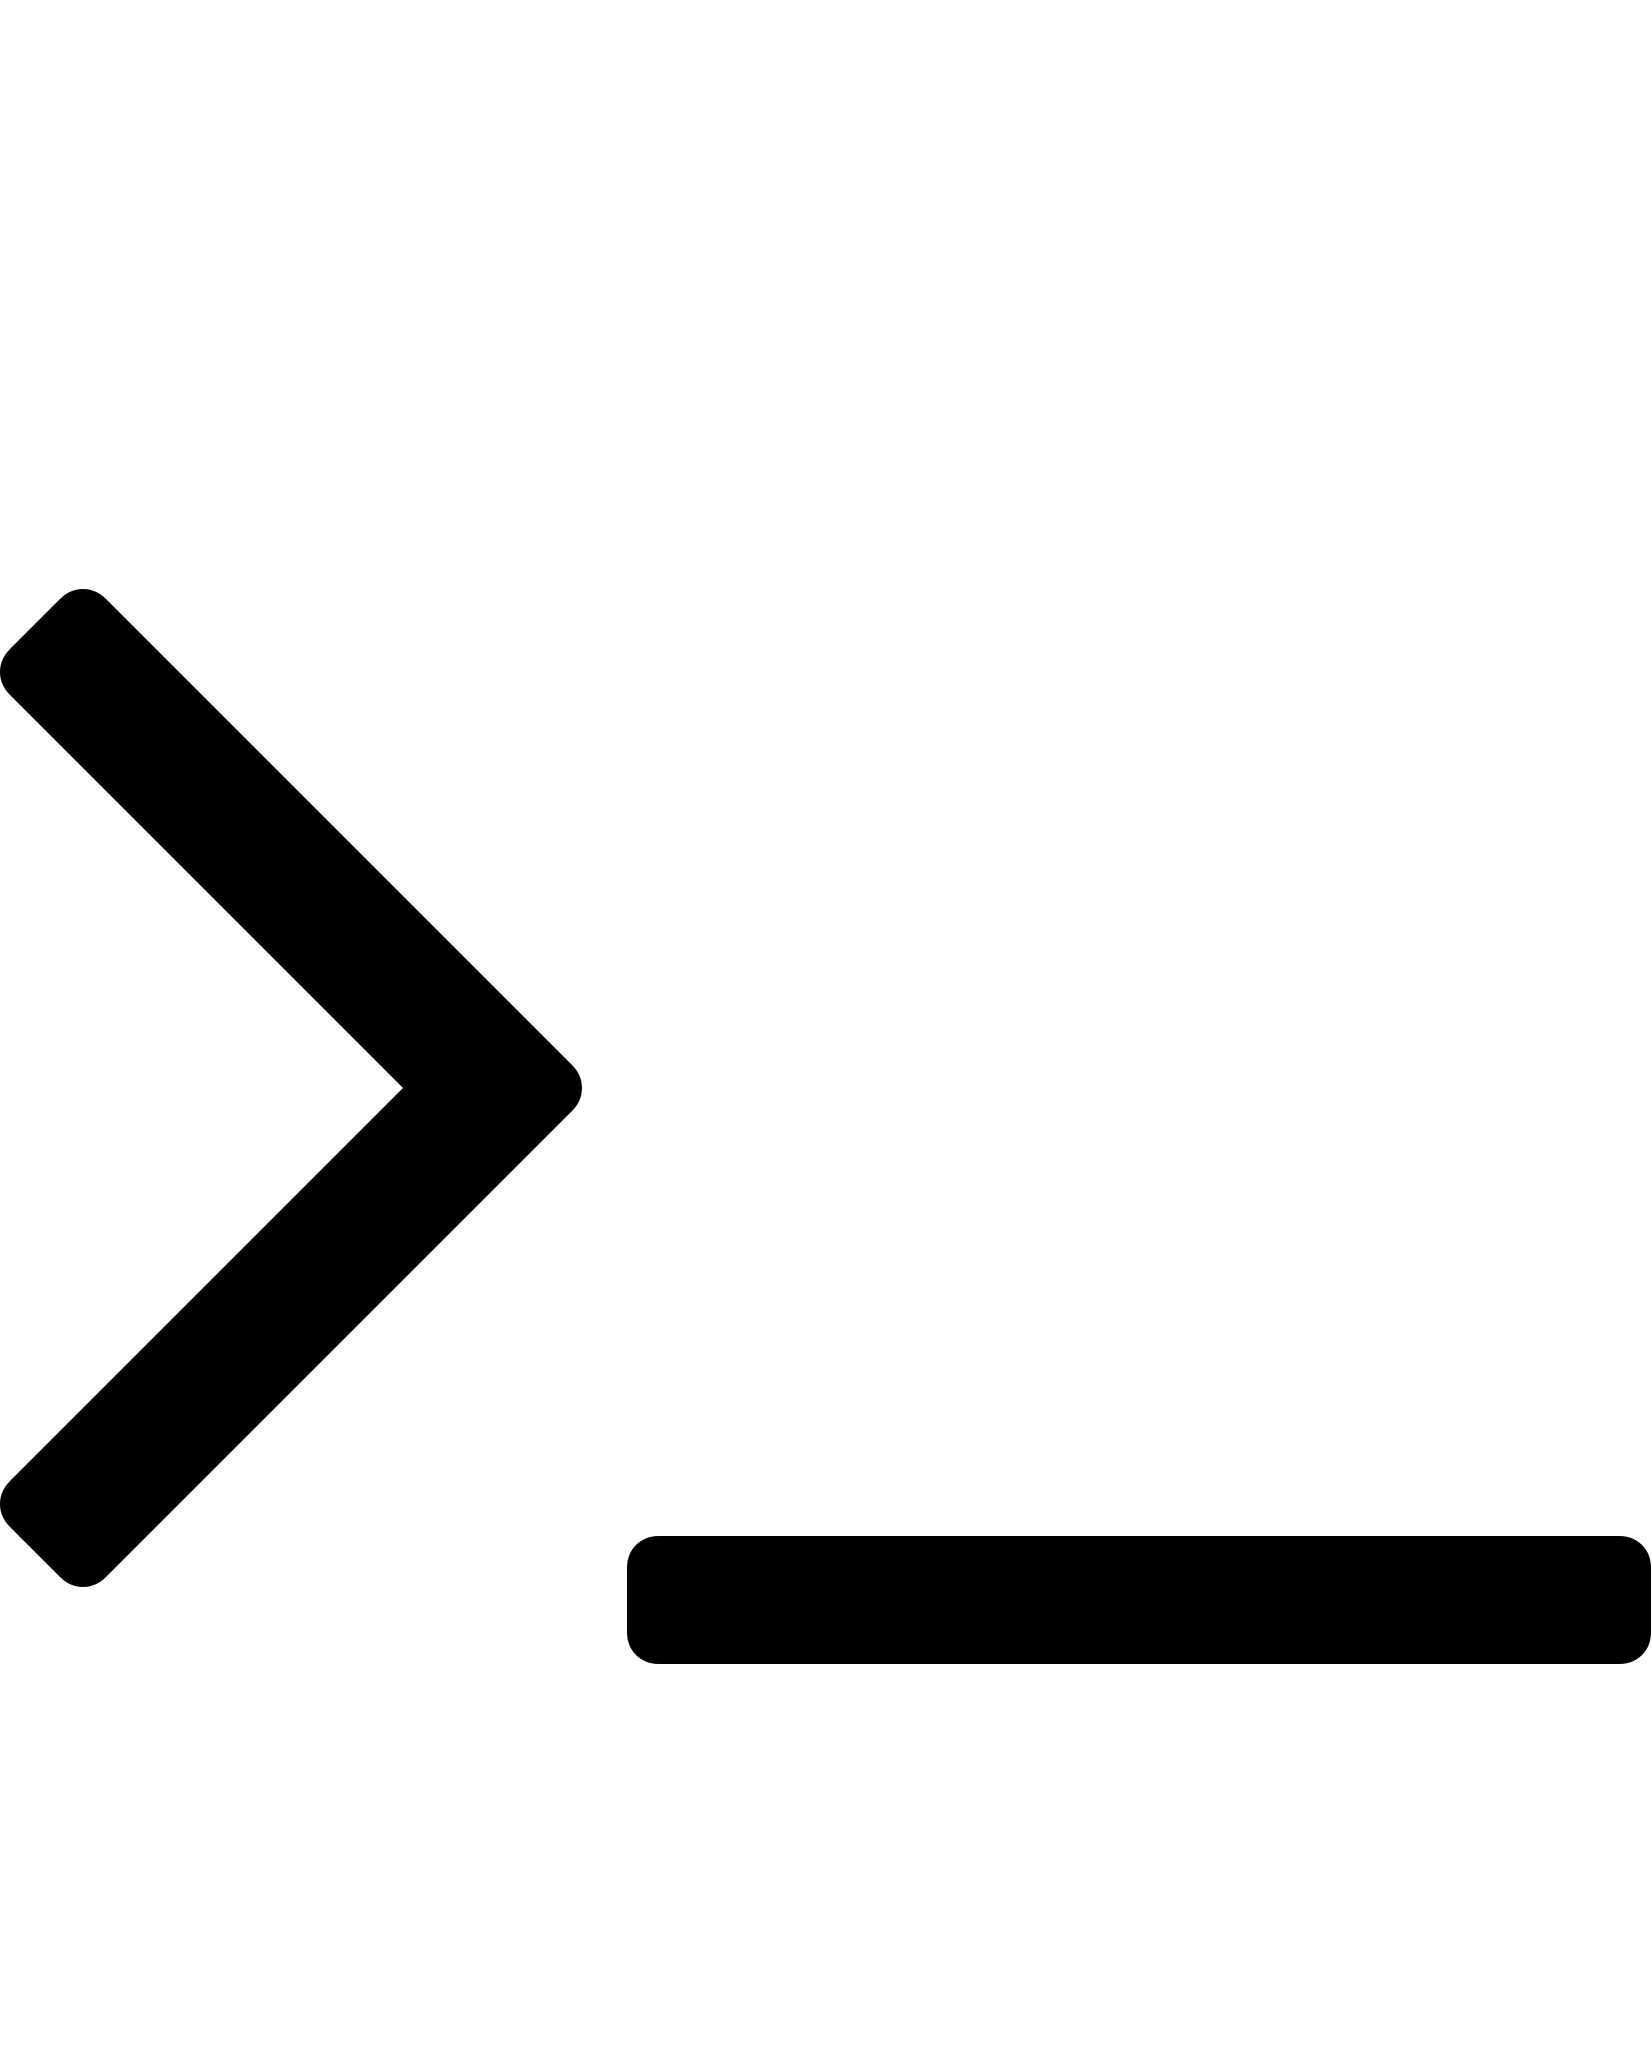
\includegraphics[width=4cm]{images/demo}
    \end{center}
  \end{frame}

  \section{Policies}
  \begin{frame}
    \frametitle{Policies}
    \begin{center}
      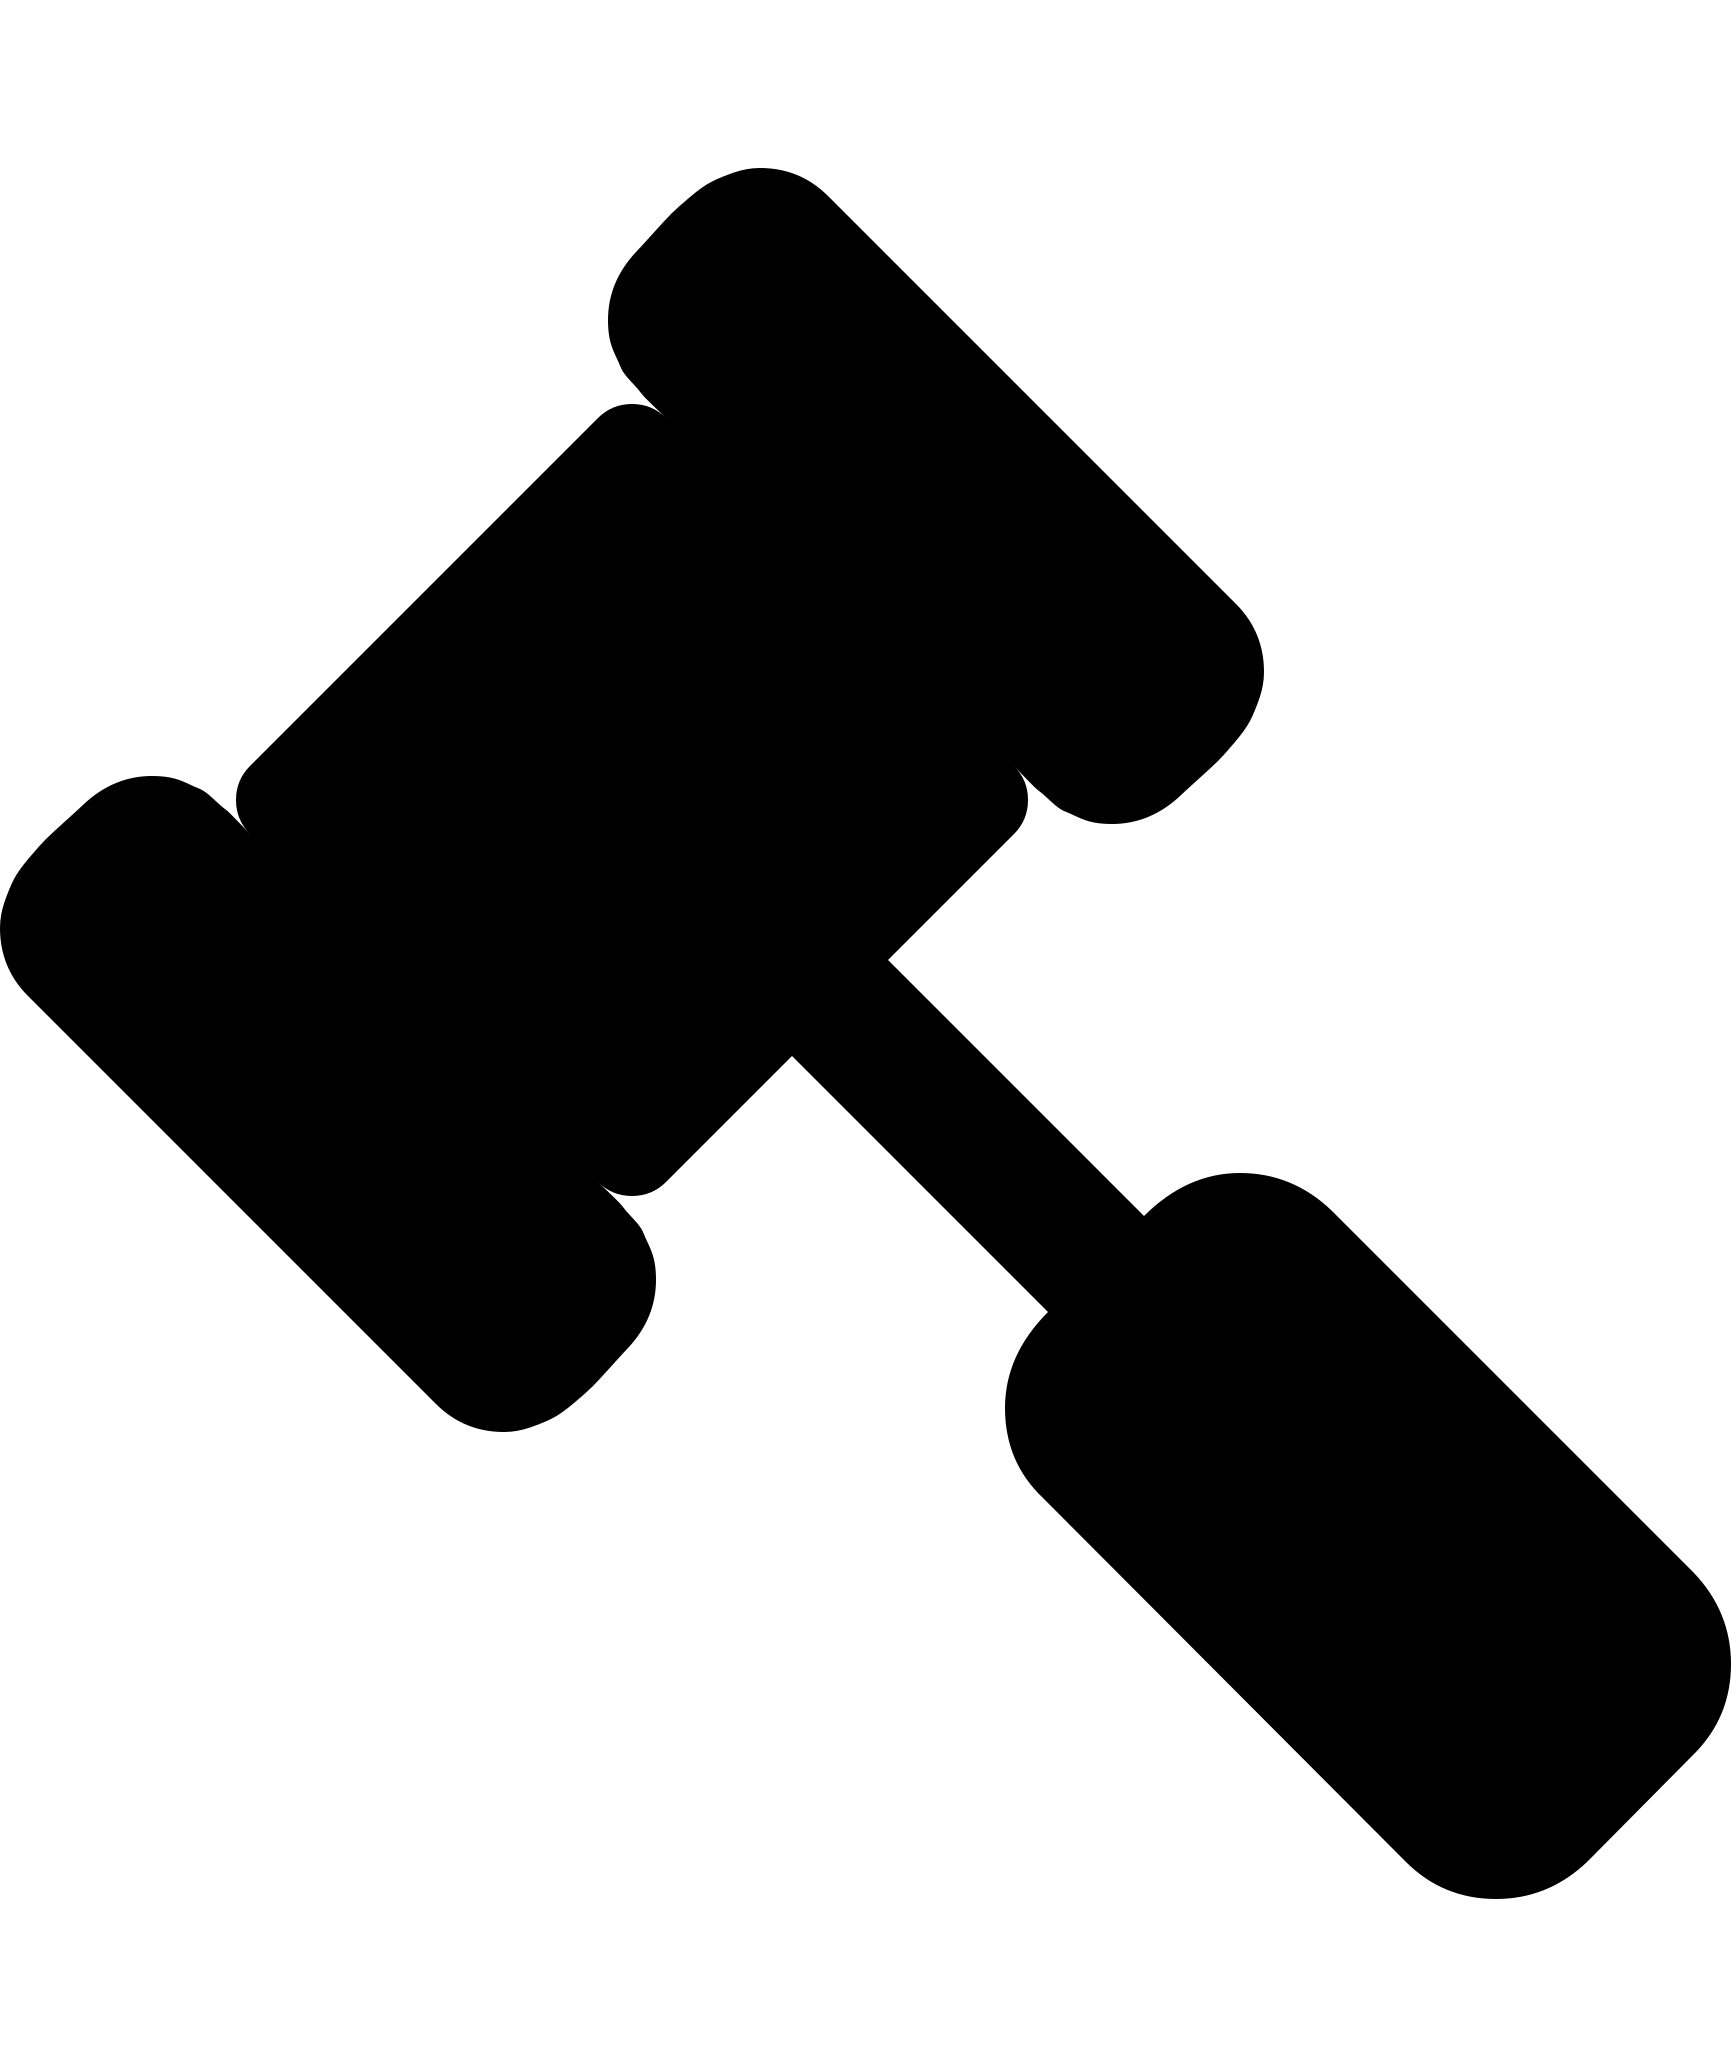
\includegraphics[width=4cm]{images/policies}
    \end{center}
  \end{frame}
  \begin{frame}
    \frametitle{Repositories}
    \begin{itemize}
      \item \emph{stable}: for stable release (link to a static archive)

        The only one interesting for the end-users.
      \item \emph{testing}: for beta versions or pre-releases
      \item \emph{unstable}: anything, even links to Git masters
      \item \emph{coqs}: Coq version for developers (branches, trunk)
    \end{itemize}
  \end{frame}
  \begin{frame}
    \frametitle{Naming scheme}
    \begin{itemize}
      \item regular expression: \texttt{coq-[a-Z0-9\textbackslash-]+}
      \item example: \texttt{coq-ssreflect}
      \item prefix \texttt{coq-} to distinguish from OCaml packages
      \item lowercase letters, dash as separator (\texttt{-}) to be uniform
    \end{itemize}
  \end{frame}
  \begin{frame}
    \frametitle{Versions scheme}
    We must be strict because people will use inequalities over version numbers for dependencies, and it has to be predictable.
    \begin{itemize}
      \item \emph{SemVer} convention: \texttt{MAJOR.MINOR.PATCH}. In theory:
        \begin{itemize}
          \item \texttt{MAJOR}: breaking changes
          \item \texttt{MINOR}: backward compatible changes
          \item \texttt{PATCH}: bug fixes
        \end{itemize}
      \item example: \texttt{1.5.1}
      \item If it is hard for your package to follow, you probably need to do some \emph{divide and conquer}.
    \end{itemize}
  \end{frame}
  \begin{frame}
    \frametitle{Versions scheme for non-stable releases}
    Recommendations: using letters:
    \begin{itemize}
      \item pre-releases: \texttt{1.6-beta1} or \texttt{1.6-rc3} (are smaller than \texttt{1.6.0})
      \item branches: \texttt{1.6.dev} (bigger than \texttt{1.6.0})
      \item master: \texttt{dev} (bigger than any version starting with a number)
    \end{itemize}
    (the order on versions in OPAM is the same as in Debian)
  \end{frame}
  \begin{frame}
    \frametitle{Build system}
    Note: \emph{OPAM is not a build system.}
    \begin{itemize}
      \item to exploit the \texttt{-j} option of OPAM, we should enforce the:
        \begin{center}
          \texttt{make "-j\%{jobs}\%"}
        \end{center}
        in OPAM files.
      \item we hope \texttt{coq\_makefile} will be enough for most of the packages
    \end{itemize}
  \end{frame}

  \section{Bench system}
  \begin{frame}
    \frametitle{Bench system}
    \begin{center}
      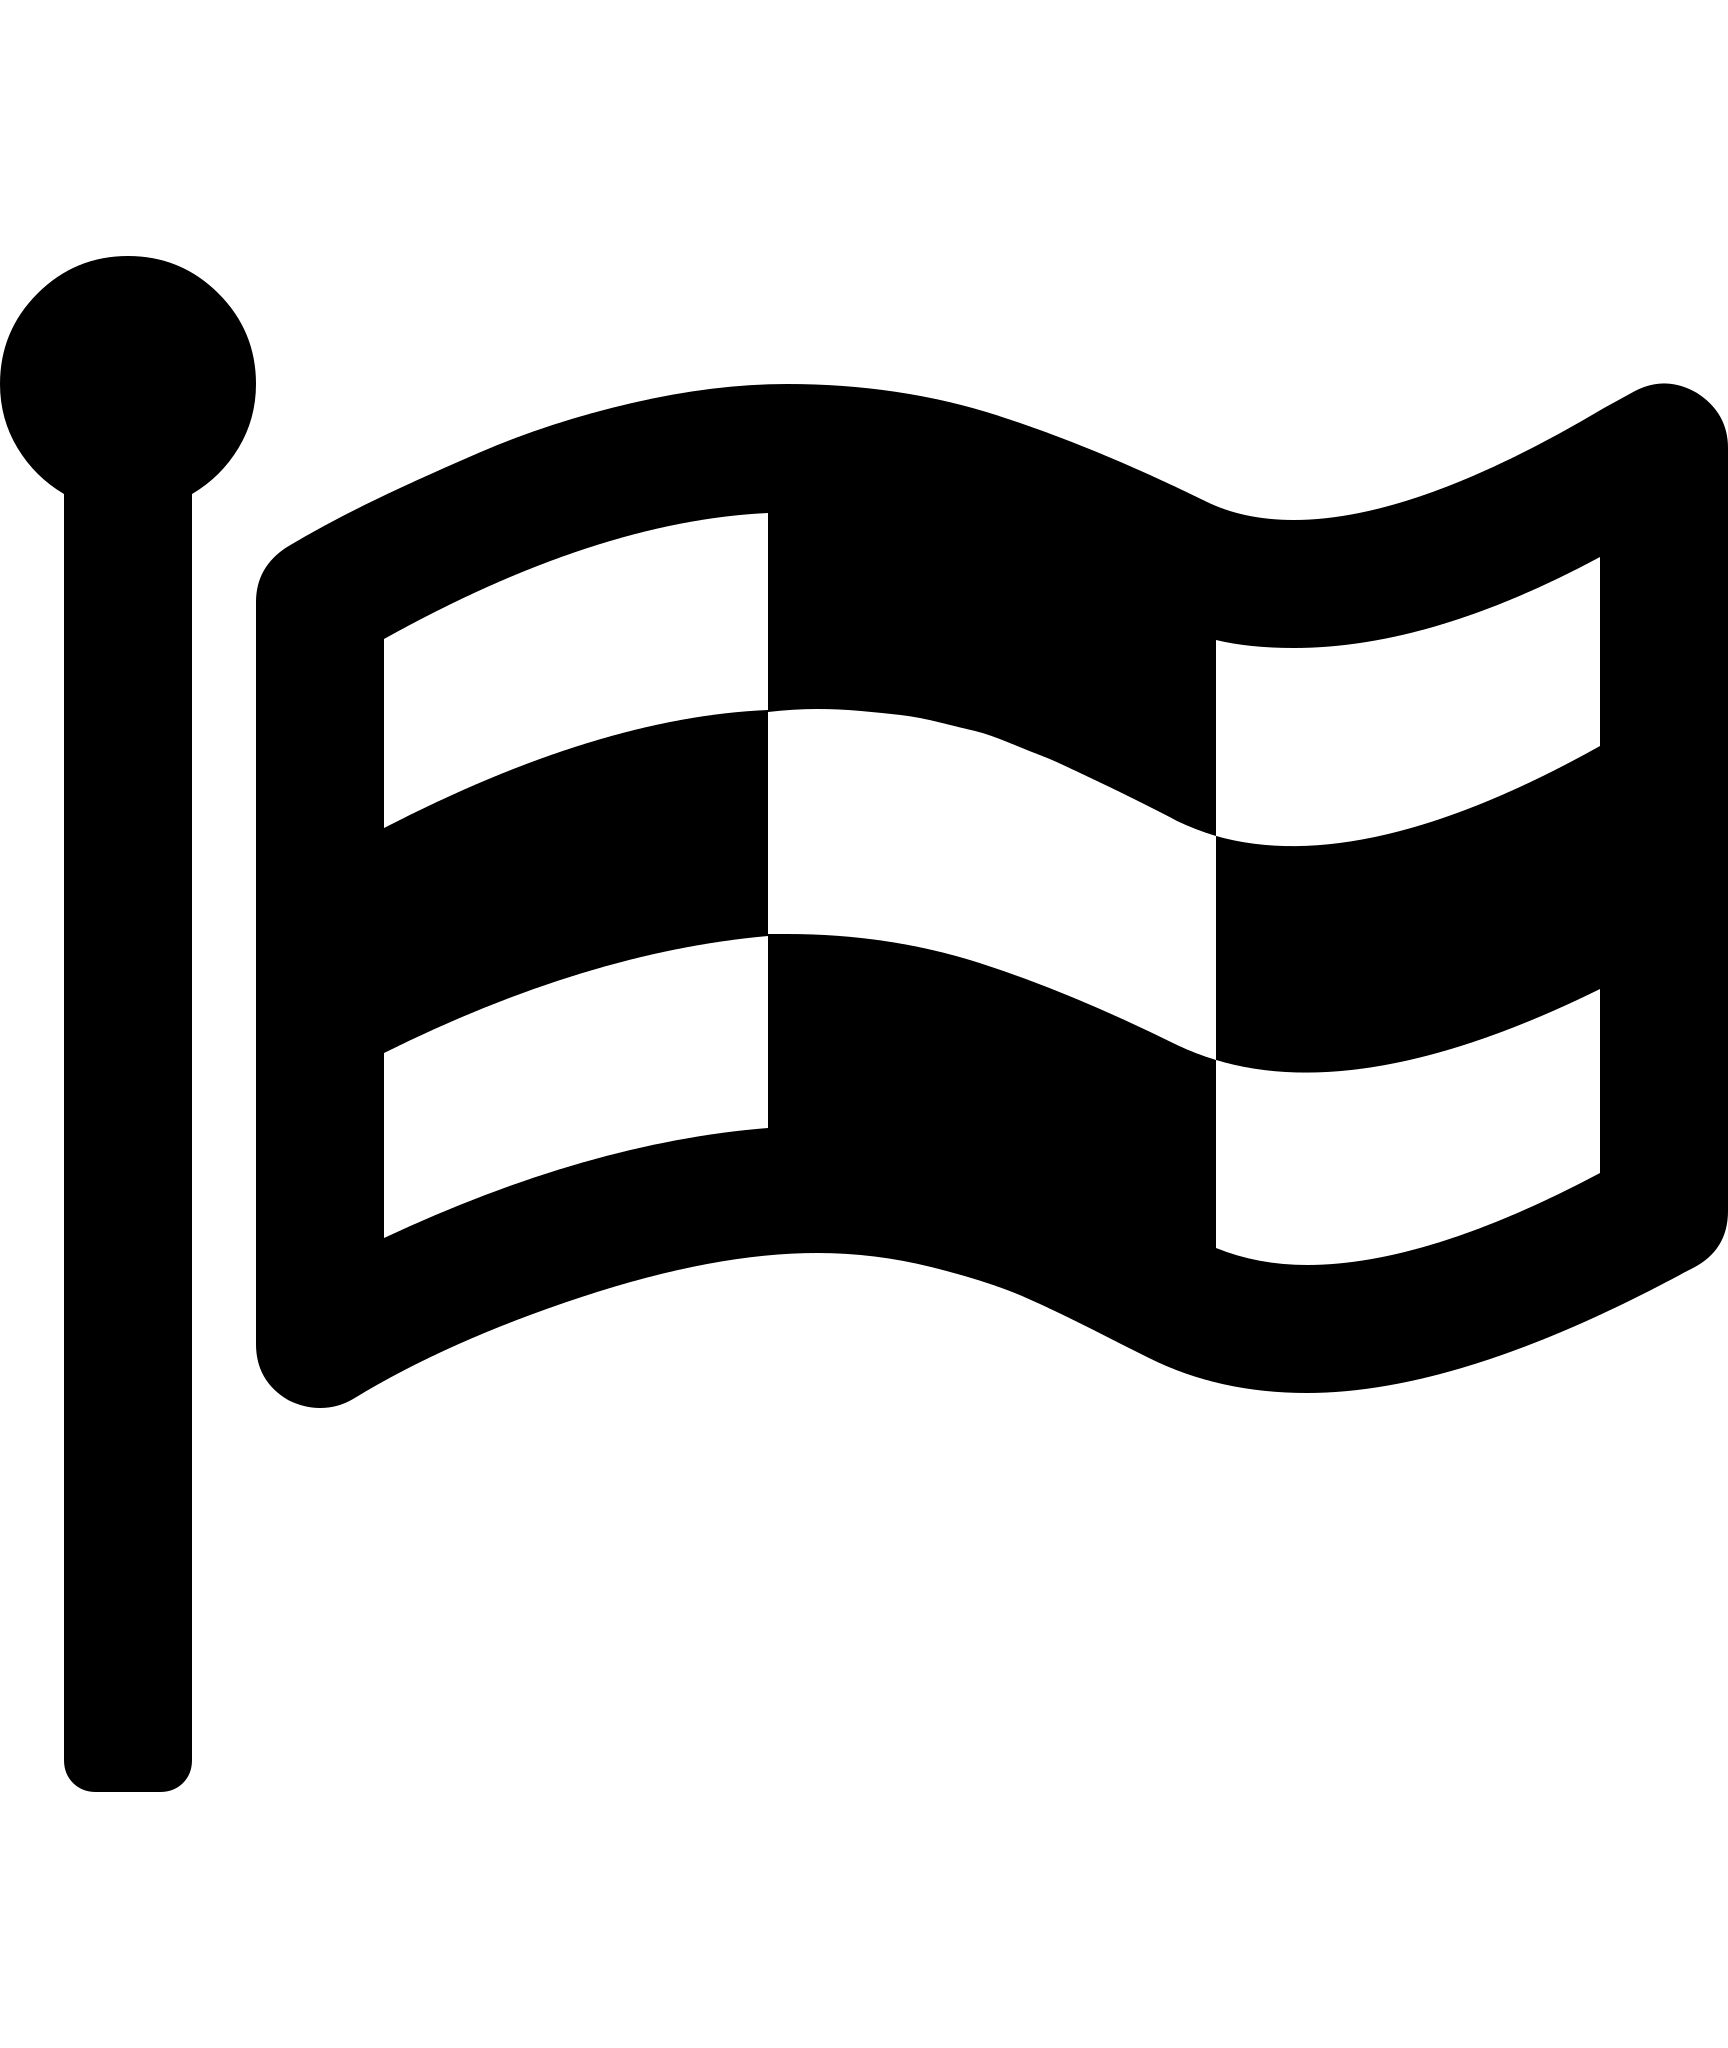
\includegraphics[width=4cm]{images/bench}
    \end{center}
  \end{frame}

  \section*{Conclusion}
  \begin{frame}
    \frametitle{TODO}
    \begin{itemize}
      \item add the OPAM website on \url{http://coq.inria.fr/}
      \item improve the bench
      \item what should we do with the \emph{contribs}?
    \end{itemize}
  \end{frame}
  \begin{frame}
    \frametitle{Thanks.}
    \Huge{Thanks.}
  \end{frame}
\end{document}
